\documentclass[11pt,a4paper,leqno]{article}
\usepackage{a4wide}
\usepackage[T1]{fontenc}
\usepackage[utf8]{inputenc}
\usepackage{float, afterpage, rotating, graphicx}
\usepackage{longtable, booktabs, tabularx}
\usepackage{verbatim}
\usepackage{eurosym, calc, chngcntr}
\usepackage{amsmath, amssymb, amsfonts, amsthm, bm, delarray}
\usepackage{caption}

% \usepackage[backend=biber, natbib=true, bibencoding=inputenc, bibstyle=authoryear-ibid, citestyle=authoryear-comp, maxnames=10]{biblatex}
% \bibliography{bib/hmg}

\usepackage[unicode=true]{hyperref}
\hypersetup{colorlinks=true, linkcolor=black, anchorcolor=black, citecolor=black, filecolor=black, menucolor=black, runcolor=black, urlcolor=black}
\setlength{\parskip}{.5ex}
\setlength{\parindent}{0ex}

\theoremstyle{definition}
\newtheorem{exercise}{Exercise}
\renewcommand{\theenumi}{\roman{enumi}}

% Set this counter to "first exercise of the week minus one".
\setcounter{exercise}{0}

\begin{document}

\begin{center}
    \begin{large}
        \textbf{
            Effective programming practices for economists\\
            Universität Bonn, Winter 2021/22 \\[2ex]
            Exercise solution\\[2ex]
            Gewei Cao, Yuhsin Chen, Xinyue Wang, Yingyu Wu, Zihan Yang
        }
    \end{large}
\end{center}


\begin{exercise}
    ~ % do not delete this innocent tilde unless you put text here
    \begin{enumerate}
        \item The advantages of splitting up the code:\par
        By decomposing the code in a certain way, it is clearer and more flexible to manage for larger projects.
After splitting the code into repositories according to a certain logic, the repositories and modules have self-describing features, so that developers working together can understand them at a glance. At the same time, the impact of some “bad code” will be contained in a certain repository, without affecting the entire project code.
        \item  The definition of “state” in a programming context:\par
        The stored inputs in a computer program are stored as variables or constants. In analyzing the state of a program, developers may go through and look at values that are stored in these inputs. As the program is executed, its state may change — variables can change and the values that are stored in memory can also change. For example, a control variable such as a variable used in a loop changes the state of the program at each iteration. Looking at the state of a program can be considered a testing method or a way of analyzing the code base.
        \item Explain the side effect of functions and why it should be avoided:\par
        A side effect is when a function relies on, or modifies, something outside its parameters to do something. For example, a function which reads or writes from a variable outside its own arguments, a database, a file, or the console can be described as having side effects. Functions with side effects especially when it is unintended could lead to a lot of potential bugs which are harder to debug.\par
For example, side effect may change the binding of a variable defined outside the local namespace.
Python searches in four namespaces when a variable is used: local, enclosing, global and built-in. The namespaces are searched in this order until the name is found and if not found Python raises a NameError exception. We will not cover all pesky details of namespaces but instead focus on the global and local namespace. Here is the specific example:\par
\begin{center}
    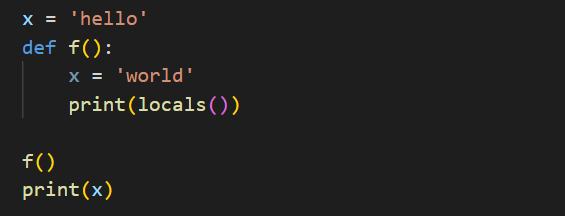
\includegraphics[scale=0.8]{example1.png}
\end{center}
prints\par
\begin{center}
    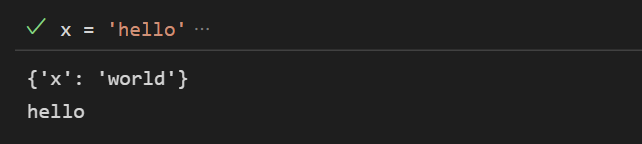
\includegraphics[scale=0.8]{example2.png}
\end{center}
The reason is that inside the function we create a new string object and bind a hello variable named x to it as also seen by the output of the locals()function. The world variable x is kept bound to the string 'world' as we would have expected. Contrast the above with the following:\par
\begin{center}
    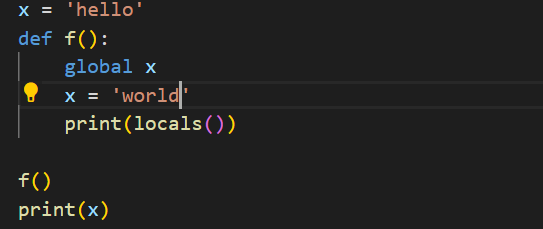
\includegraphics[scale=0.8]{example3.png}
\end{center}
that prints\par
\begin{center}
    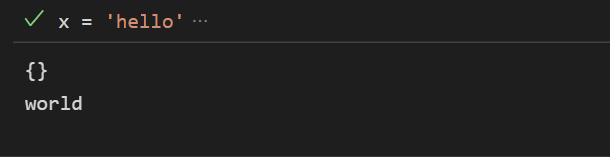
\includegraphics[scale=0.8]{example4.png}
\end{center}
We can see that the variable x outside the function is now bound to the string object created within the function. This is a side effect and a prime example of things to avoid. The same can be achieved by directly accessing the globals dictionary. In fact it is not even necessary to bind the variable x before the function is called:\par
\begin{center}
    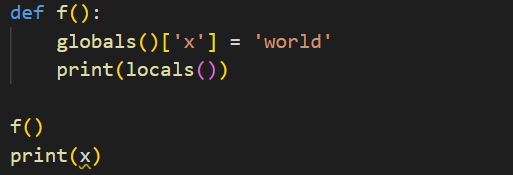
\includegraphics[scale=0.8]{example5.png}
\end{center}
prints\par
\begin{center}
    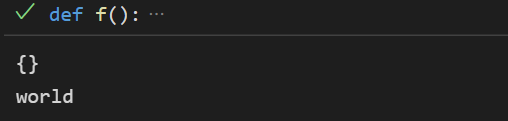
\includegraphics[scale=0.8]{example6.png}
\end{center}
\item The uses of map, filter and reduce and their same style:\par
It is a programming approach in which a program is written with a view of describing
WHAT it has to do / WHAT problem it is intended to solve rather than how it should solve the problem.
Declarative programming approaches do not describe the control flow in detail.

Imperative Programming is a programming approach where the program's control flow is explicitly written.
It mentions HOW a problem should be solved / HOW a task should be done.Here is the example:
% map function:
The map function takes an iterable and returns a map object (another iterable) after applying a given function.
\begin{center}
    \begin{verbatim}
nums = [1, 2, 3, 4]

def map_function(function, iter_list):
    lst = []
    for i in iter_list:
        lst.append(function(i))
    return lst

cube_nums = map_function(lambda x : x*x*x, nums)

print(cube_nums)

    \end{verbatim}
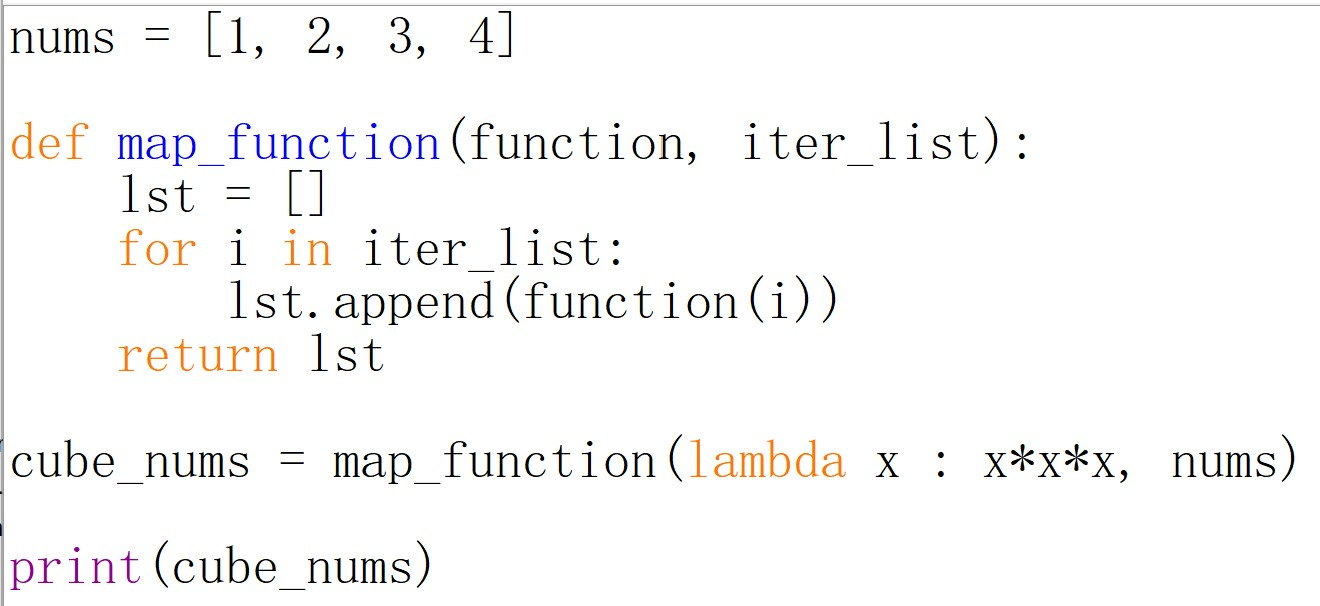
\includegraphics[scale=0.5]{map.jpg}
\end{center}
%reduce function
The reduce function takes as iterable and recursively processes the contents of it to reduce them into one value.
\begin{center}
    \begin{verbatim}
nums = [1, 2, 3, 4]

def reduce_function(function, iter_list):
    value = iter_list[0]
    for i in iter_list[1:]:
        value = function(value, i)
    return value

sums = reduce_function(lambda x, y: x + y, nums)

times = reduce_function(lambda x, y: x*y, nums)

print(sums)

print(times)
    \end{verbatim}
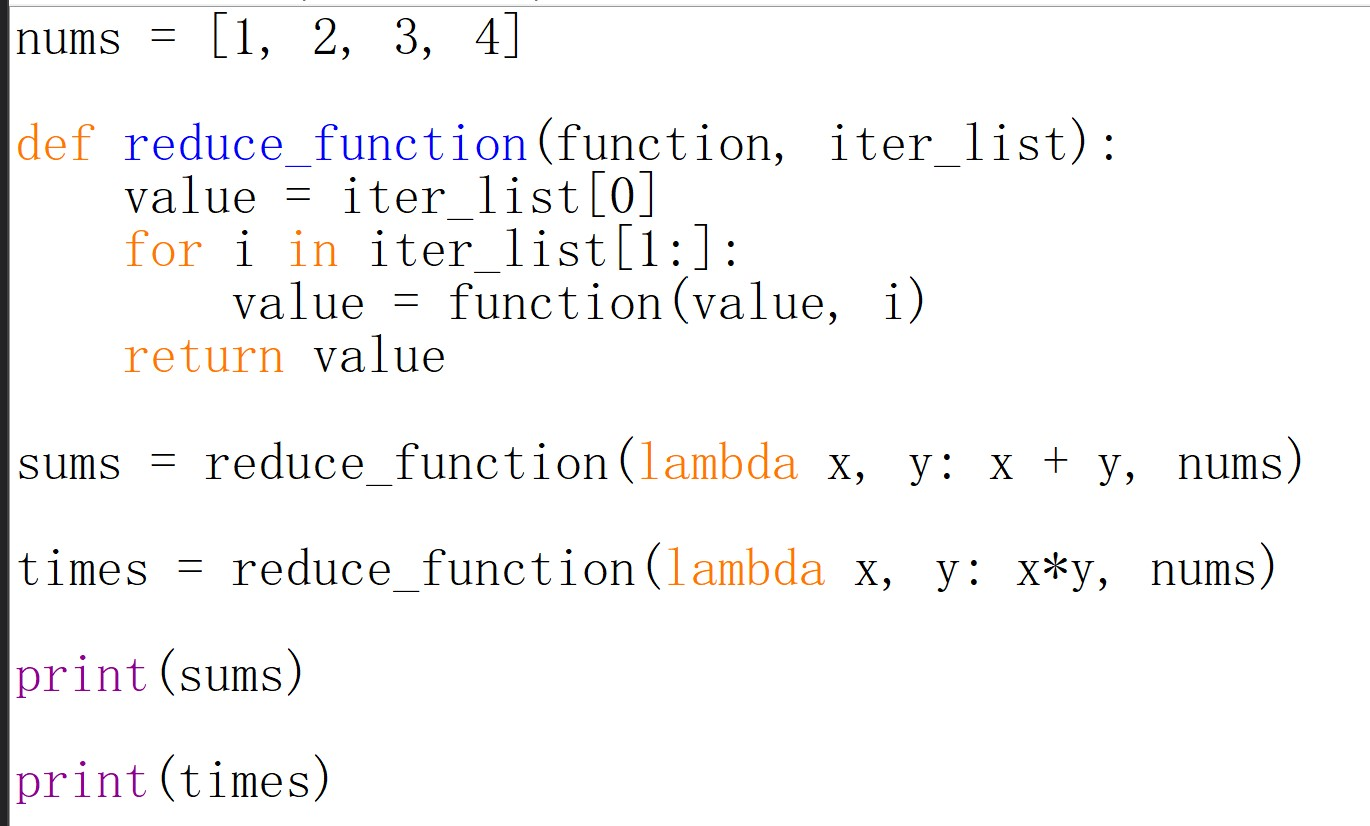
\includegraphics[scale=0.5]{reduce.jpg}
\end{center}

%The filter function
The filter function takes an iterable and filters it according to a given function.
\begin{center}
    \begin{verbatim}
nums = [1, 30, 59, 67, 64, 114, 51, 4, 74]

def filter_function(function, iter_list):
    lst = []
    for i in iter_list:
        if function(i) == True:
            lst.append(i)
    return lst

filterd = filter_function(lambda x: x >= 50, nums)

print(filterd)
print(nums)
    \end{verbatim}
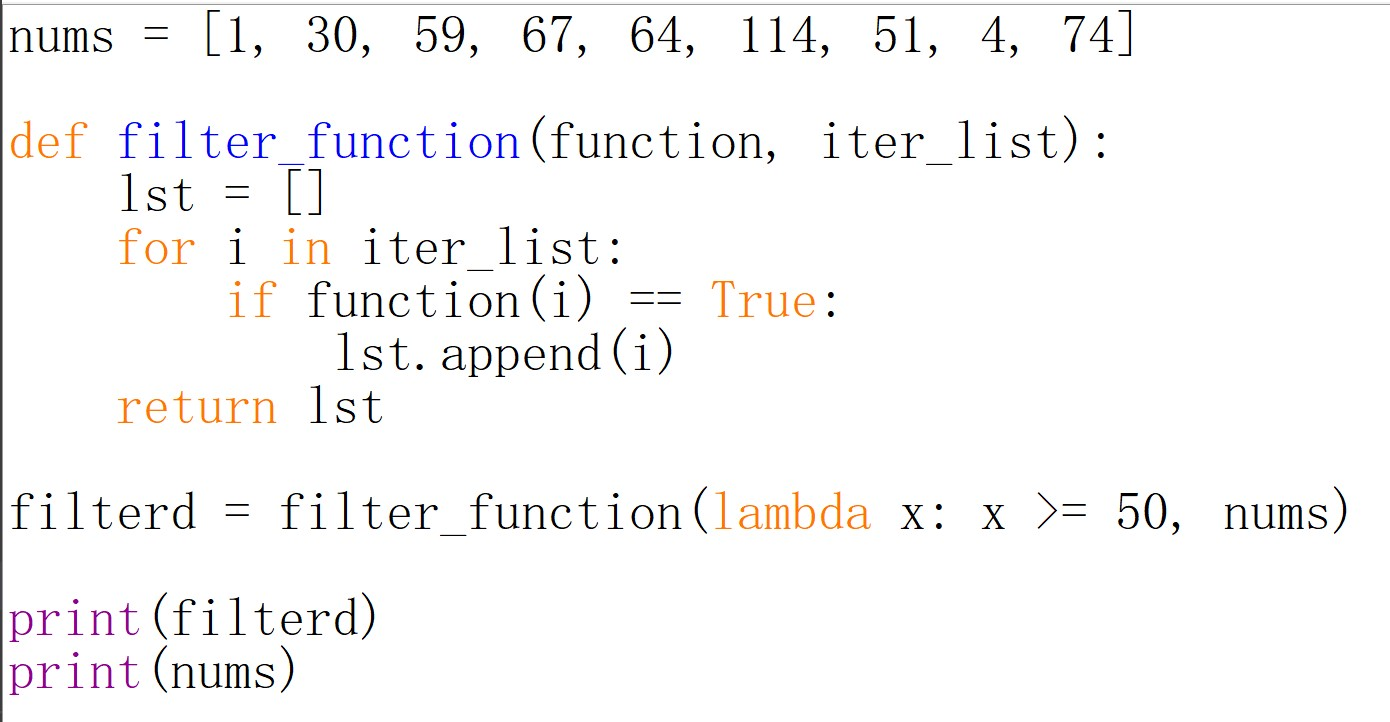
\includegraphics[scale=0.5]{filter.jpg}
\end{center}

    \end{enumerate}
\end{exercise}


% \printbibliography

\end{document}
